%! TEX root = ../aminhash.tex

% Discuss results
% Explain conflicting results, unexpected findings and discrepancies with other research
% State limitations of the study
% State importance of findings

\section{Conclusion}

We have shown that it is possible to substantially improve upon the traditional MinHash estimator in the database or one-way communication setting.
Our analysis has shown one can reduce the global risk by nearly 30\%,
and much more when the size of the sets differ.
%The fact that our variance is $\frac{n_y}{n_x+n_y}$ of MinHash's variance suggests that our method might be particularly useful for containment queries, in which the 
Meanwhile, our experiments have shown a similar improvement in recall on standard datasets.

While our first estimator had a running time of $\Omega(K \min\{|X|,|Y|\})$, can be slow, we derived a faster $O(K)$ time estimator, which has a similar variance and often even an improved recall.
%The Minner estimator with newton=8 can sometimes give results quite different from MLE, because of the approximation into making it linear.
The success of our Minner estimator also suggests that the count of ``hash values smaller than the minimum'' could be used more widely.
Perhaps as part of the input supplied to Machine Learning pipelines working with coordinated sampling.

While our estimator only takes time $O(k)$ per data point, they do however still need to do at least two table lookups per value, where the classical estimator just needs to do a single equality comparison.
In \cref{sec:alg} we discussed how the table lookups could be done using fast SIMD instructions, as is done in the Product Quantization world, which presumably would close the remaining gap.
%Ideally our algorithm runtime should be dominated by loading data from memory into cache/registers.

\section{Open Problems}

Besides the SIMD considerations in \cref{sec:alg}, there are a number of potential future directions:
\begin{enumerate}
   \item Weighted MinHash~\cite{ioffe2010improved} And ``Probability MinHash''~\cite{moulton2018maximally} are common extensions of MinHash to non-binary data.
      As with classical MinHash all known estimators follow the symmetric paradigm, so could potentially see similar improvements to what we have shown in this paper.
%   \item Bottom-$k$ MinHash has often been shown to give better estimates than the $K$ independent hash functions MinHash we have studied.
%      Bottom-$k$ also has the benefit of faster hashing, which would translate to faster index generation time in the database setting.
%      The approach has nice combinatorial properties that might also lead to fast estimators.
   \item Is the Minner Estimator consistent? In \cref{sec:minner} we gave results that indicate Minner may not be unbiased.
      However, experimentally it appears to converge to the right value as $K\to\infty$.
   \item Use a Bayesian prior for $Y$.
      In \cref{sec:mle} we briefly discussed the possibility of assuming a prior on $Y$ other than the uniform distribution.
      Since all the datasets of Mann et al.~\cite{mann2016empirical} have some elements of the domain more common than others (and the Flickr dataset particularly so), such a prior, based on statistics on the dataset, could potentially be very efficient.
   \item Finally we suggest the task of finding the best possible sketch for sets in general.
      In~\cite{DBLP:conf/focs/AhleK20} it was shown that a best possible space partition exists for set similarity search with any set similarity measure.
      One could imagine a similar result, which would replace MinHash as the preferred quantization method for sets.
\end{enumerate}

% \begin{acks}
% Rasmus Pagh and Ninh Pahm
% \end{acks}


\begin{figure}
   %\hspace{-1em}
   \centering
   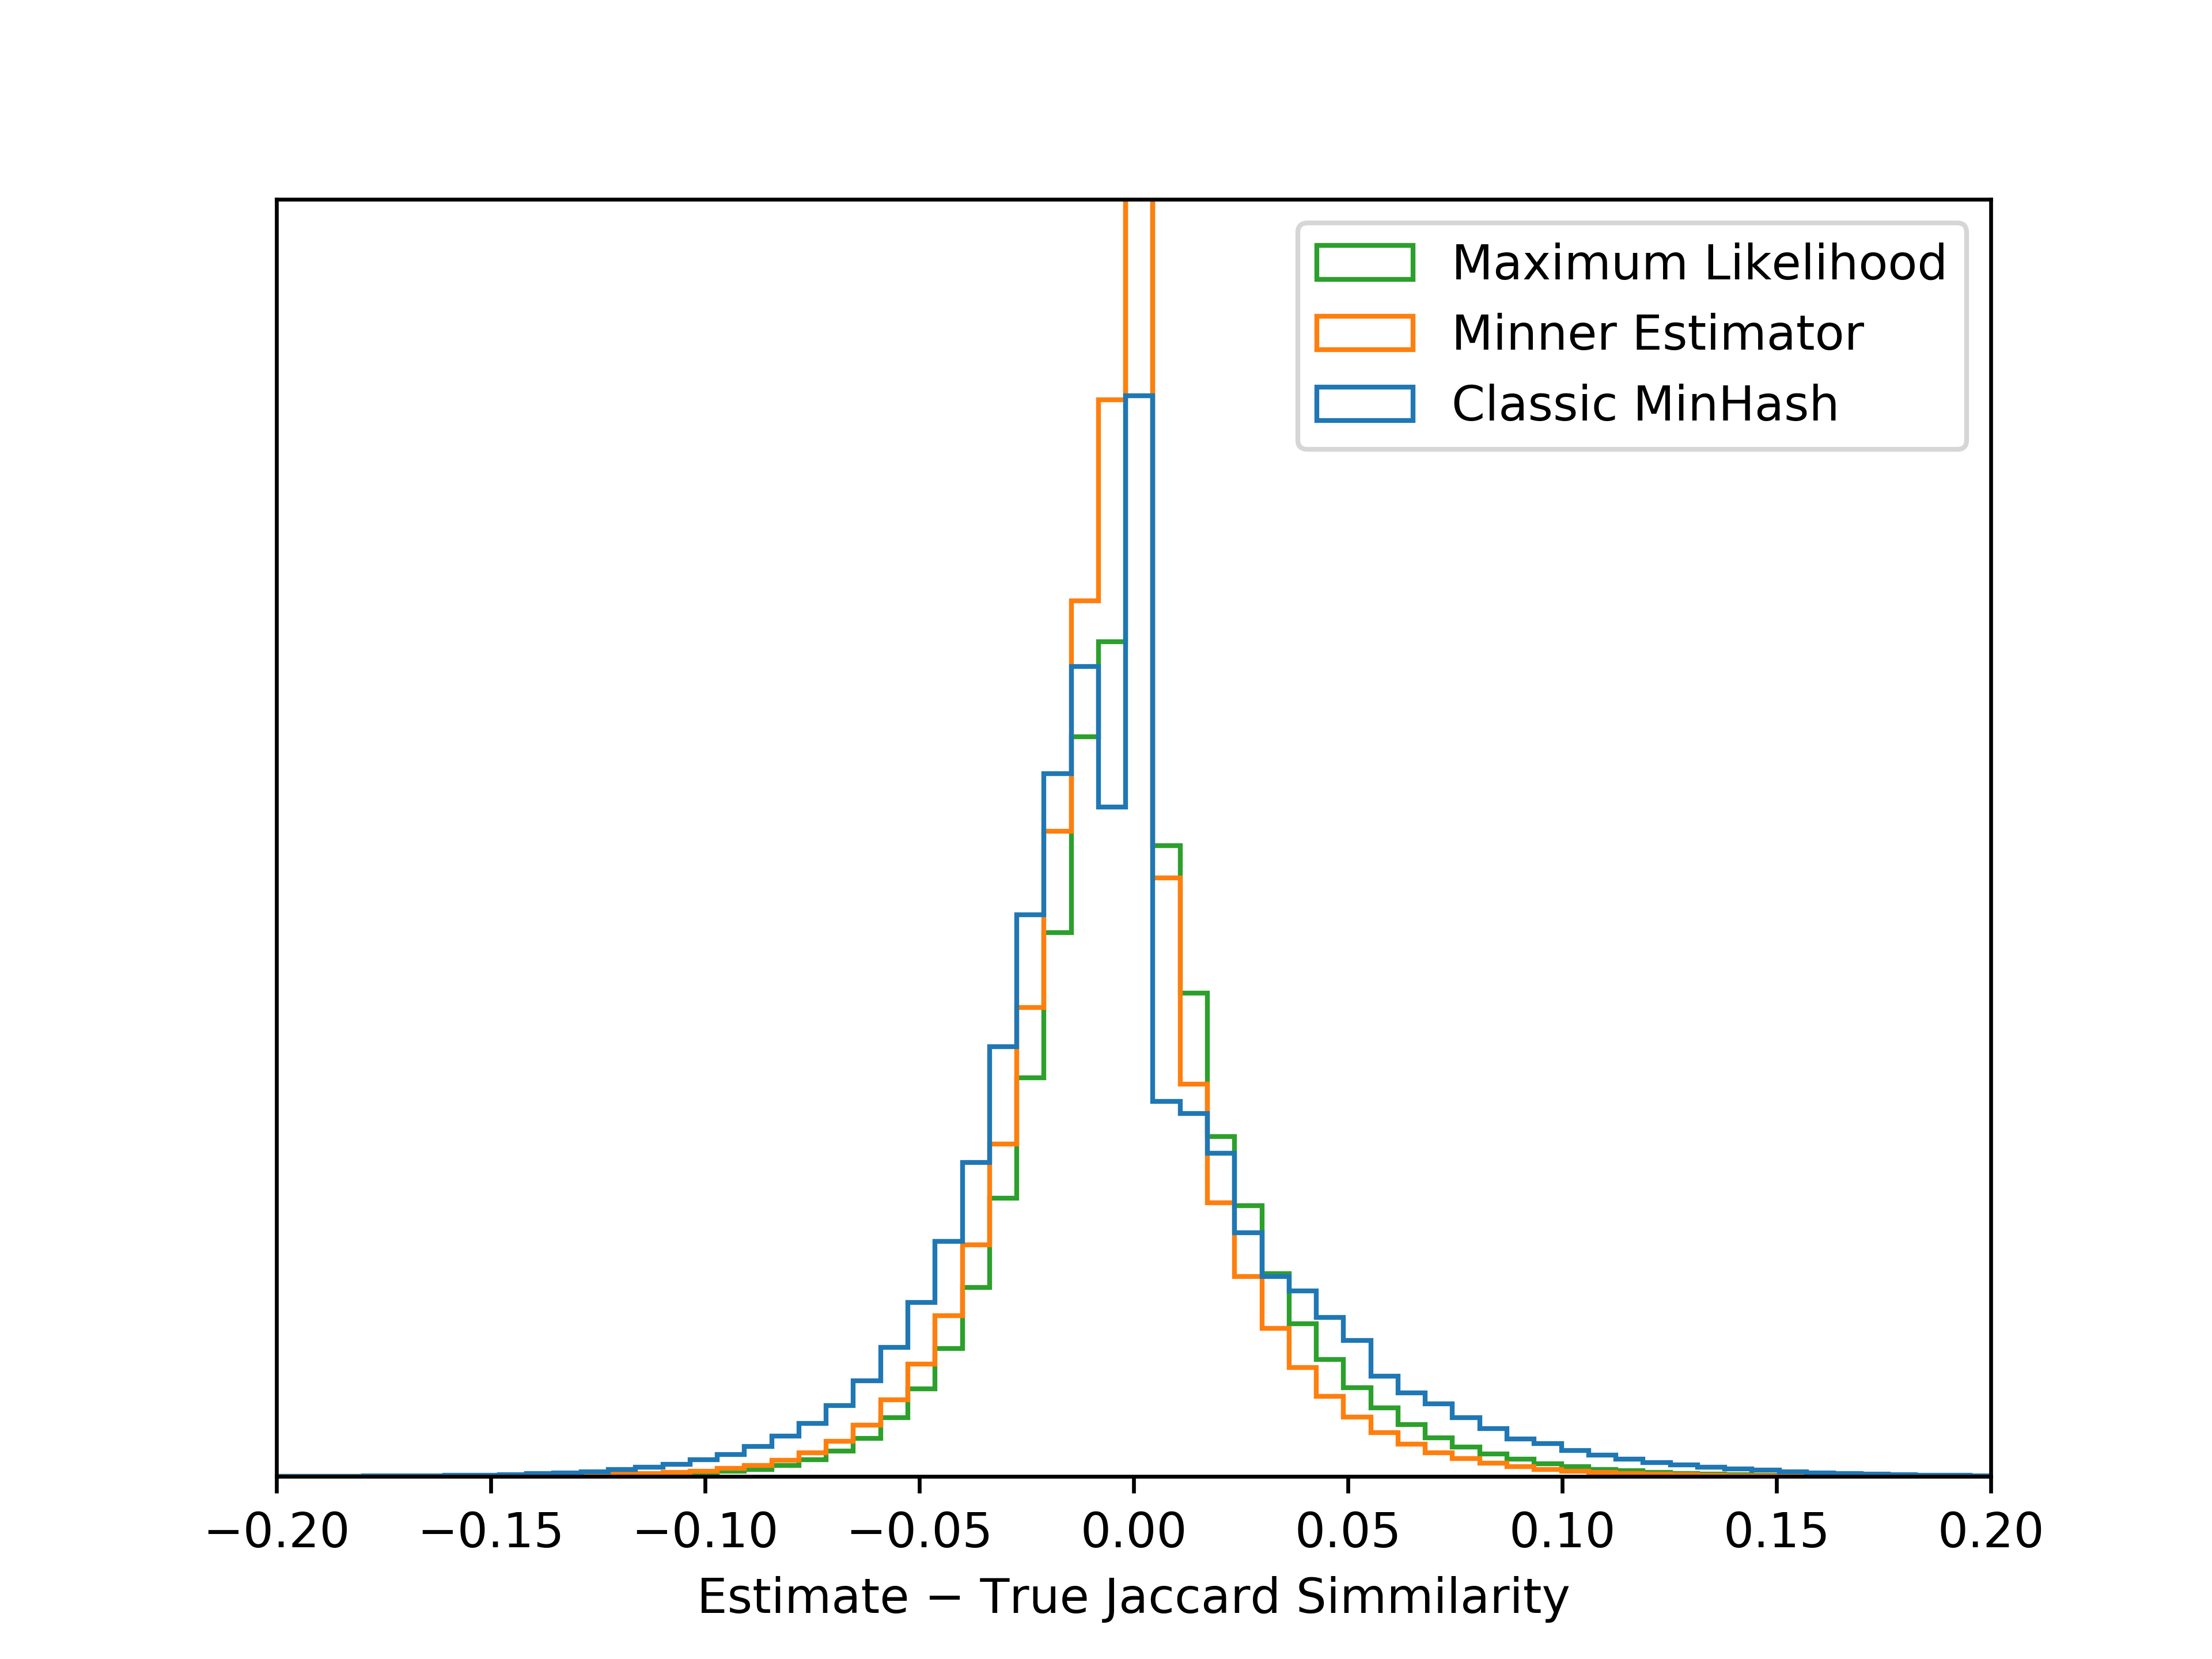
\includegraphics[trim=0 5 35 40,clip,width=\linewidth]{figures/hist2}
\caption{The density of estimation errors on Netflix dataset at $K=31$ over a million pairs.
%The empiric means are $0.0114$ for the symmetric estimator, 
%$0.0002$ for the Minner estimator, and 
%$0.0038$ for the Maximum likelihood estimator.
Besides a slightly better variation, the maximum likelihood estimator has a much better chance of getting a ``perfect'' estimate.
%The top of the plot has however been cut off so one can see the bottom more clearly.
}
\end{figure}

